\documentclass[11pt,a4paper]{article}
\usepackage[margin=2.2cm]{geometry}
\usepackage{graphicx,booktabs,url,amsmath}
\usepackage[hidelinks]{hyperref}
\graphicspath{{../../../fullsim_analysis/results/bench/2026-10-21/}}
\title{Bench data of 21 October 2026: first look}
\author{J. J. G\'omez-Cadenas}
\date{22 October 2026}
\begin{document}
\maketitle

Data measured by Laura Navarro on 21 October 2026 with the A5202 (board 0) and the PET CAEN
DAQ, copied from \path{hyperion:/data/lnavarro/26_10_caen_measurements_jj}. The runs follow
bench note 1 (Citiroc noise). Channels are numbered 0--63 as in the DAQ.

\section{Data received}

\begin{center}
\small
\begin{tabular}{lp{0.62\textwidth}l}
\toprule
Item & Content & Logbook \\
\midrule
run-1 \ldots\ run-9 & decoded events, histograms, manifest; about 10\,000 periodic triggers (1 ms) each & yes \\
scan-10 & staircase, TD coarse threshold 150--300, step 1 & no \\
scan-11 & staircase, TD coarse threshold 0--600, step 2 & no \\
hold-scan-12 & hold delay 0--248 ns, step 8 ns, 10\,000 events per point & no \\
\bottomrule
\end{tabular}
\end{center}

\noindent The \path{staircase.h5} artifacts of scans 10 and 11 were not in the directory; the
same numbers are in their \path{points.jsonl}, which is what was read.

\section{Runs 1--9 and hold scan 12: every value at full scale}

\begin{center}
\small
\begin{tabular}{lllllll}
\toprule
Run & Step & HG shaping & HoldDelay & $T$ detector & $T$ board & HV current \\
\midrule
1, 2, 3 & 1 & 25, 50, 87.5 ns & 0 ns & 24.8 $^\circ$C & 50.0--50.5 $^\circ$C & 0.3--0.4 $\mu$A \\
4--8 & 2 & 25 ns & 96, 200, 296, 400, 496 ns & 24.7 $^\circ$C & 50.5 $^\circ$C & 0.3 $\mu$A \\
9 & 3 & 25 ns & 0 ns & 24.7 $^\circ$C & 50.5 $^\circ$C & 0.3 $\mu$A \\
\bottomrule
\end{tabular}
\end{center}

No trigger was lost and all 64 channels are present in every event. \textbf{But every
measurement of every channel, in the high and the low gain, is 8191}, the full scale of the
13-bit ADC, in all nine runs and at all 32 points of the hold scan. 

The setup appears to be correct. The DAQ stores the configuration that
was requested and the one the board applied, parameter by parameter; the audit marks every
parameter as applied, and all of them agree with the settings table of bench note 1 except
\texttt{HV\_Vbias}. The only parameter the note did not fix is \texttt{Pedestal}, which is 0.

Whatever went wrong it not recorded in the files.

There are differences between the content of the files and the logbook:
\begin{itemize}
\item The files record \texttt{HV\_Vbias} = 40.7~V (\texttt{HV\_IndivAdj} = 0,
  \texttt{HV\_Adjust\_Range} = 4.5~V); the logbook says 36.5~V. If the individual adjustment
  subtracts the full 4.5~V, the SiPMs see about 36.2~V, which agrees with the current.
\item The temperature of the logbook (50--50.5~$^\circ$C) is that of the board. The detector was
  at 24.7--24.8~$^\circ$C, the FPGA at 59~$^\circ$C, the HV module at 49--50~$^\circ$C.
\end{itemize}

\section{Staircases (scans 10 and 11)}

Figure~\ref{fig:stair} shows the rate of the timing discriminator of each channel against its
coarse threshold.

\begin{figure}[h]
\centering
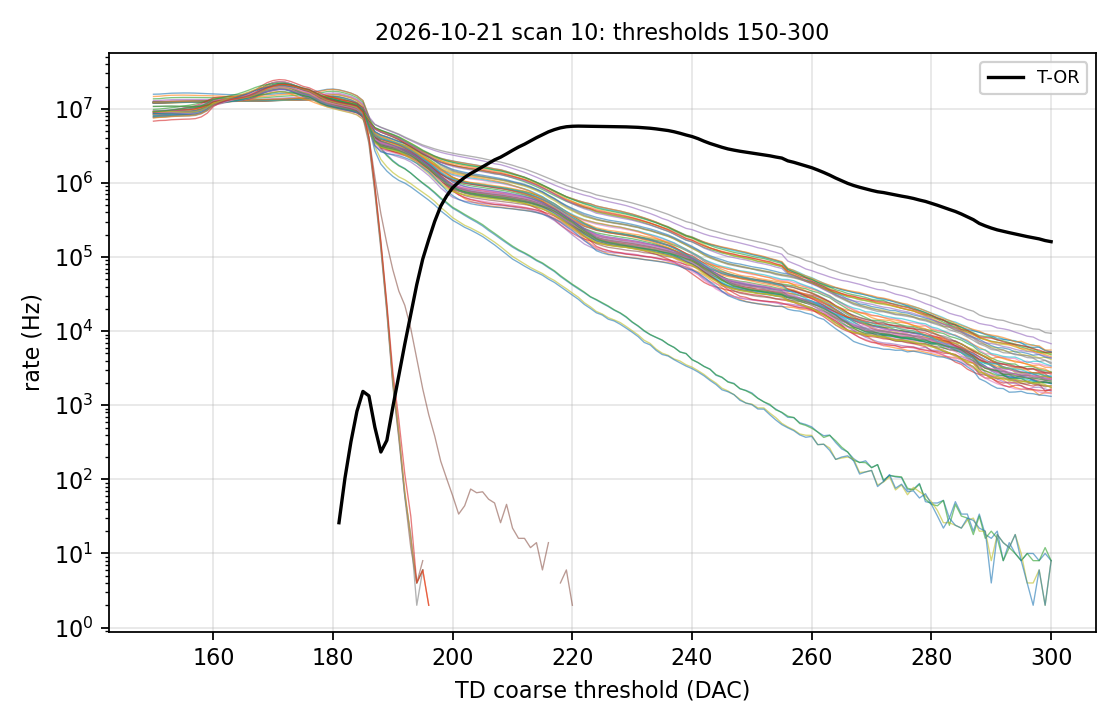
\includegraphics[width=0.49\textwidth]{staircase_10.png}
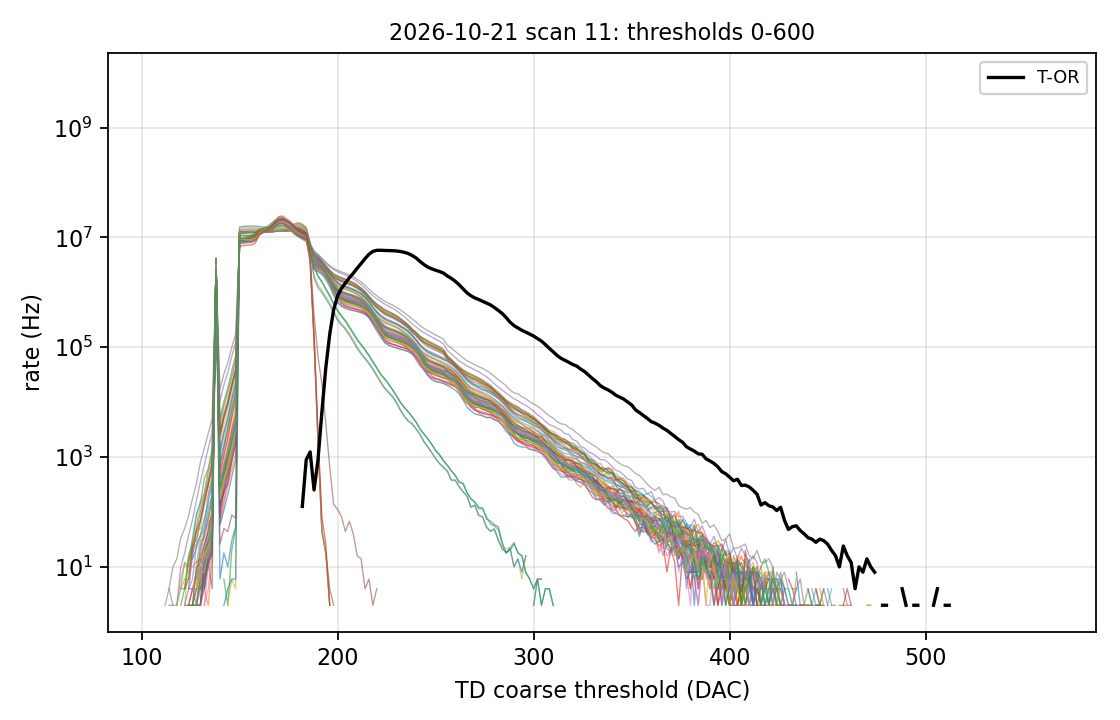
\includegraphics[width=0.49\textwidth]{staircase_11.png}
\caption{Rate of the timing discriminator against the coarse threshold, one curve per channel,
with the T-OR in black: scan 10 (left, 150--300) and scan 11 (right, 0--600).}
\label{fig:stair}
\end{figure}

\begin{itemize}
\item \textbf{Baseline.} Up to the edge of a plateau at 180--185 DAC, the same in all channels
  within 5 DAC, the rate is 1.3--2.5$\times10^7$~Hz: the threshold sits in the noise of the fast
  shaper. Below about 150 the rate drops to zero, presumably because the discriminator output
  stays high and no edge is counted.
\item \textbf{Dark counts in 54 channels.} Above the plateau the rate falls slowly and with
  shoulders: about $6\times10^5$~Hz 30 DAC above the edge (median), $10^4$~Hz near 280, 10~Hz
  near 400. This is the staircase of the dark counts (1, 2, 3 \ldots\ pe). \textbf{The SiPMs
  were therefore above breakdown during the scans}, unlike in the runs; the scan manifests do
  not record the HV.
\item \textbf{No avalanches in 6 channels: 15, 55, 57, 59, 61, 63.} Their rate falls from the
  plateau to zero within 10 DAC; 30 DAC above the edge they count 0--4~Hz.
\item \textbf{Low dark rate in 4 channels: 0, 2, 8, 10.} 60--90~kHz 30 DAC above the edge, 7--10
  times below the median. In the figure these are the isolated curves below the bundle.
\item \textbf{T-OR.} Zero below a threshold of 182, while every channel counts about
  $10^7$~Hz there; probably the OR saturates.
\item \textbf{One invalid point.} Scan 11, channel 61, threshold 490: the DAQ wrote 3735928559
  counts, i.e.\ \texttt{0xDEADBEEF}. It is left out of the figure.
\end{itemize}

The 10 channels without or with few avalanches will be a problem in what follows: if they see
no avalanches they cannot be calibrated with the periodic trigger and will not record the light
of the crystal. Five of the six silent channels are the odd channels 55--63, and the four weak
ones are even channels 0--10, which suggests a connector or a mapping rather than single SiPMs.

\section{Questions}

\begin{enumerate}
\item \textbf{(JMB?)} Why is every value 8191, in both gains and in the hold scan? Does the ADC
  not convert with this configuration (\texttt{PEAK\_STRETCH}, \texttt{Pedestal} = 0, periodic
  trigger), or does the decoder write a default? 
  \item \textbf{(JMB?)} Scan 11 contains \texttt{0xDEADBEEF} as the count of channel 61 at
  threshold 490: where does it come from?
\item \textbf{(Laura)} review the sequence of data taking: what was done
  on the board and in the DAQ before the runs, what was changed before the scans (in
  particular the HV), etc.
\item \textbf{(Laura)} What voltage does each SiPM see with \texttt{HV\_Vbias} = 40.7~V and
  \texttt{HV\_IndivAdj} = 0: about 36.2~V?
\item \textbf{(Laura)} Are SiPMs connected to channels 15, 55, 57, 59, 61 and 63? Is anything
  different about 0, 2, 8 and 10 (connector, position in the array)?
\item \textbf{(Laura)} The logbook needs rows for scans 10, 11 and 12 (time, settings, HV),
  with the temperature of the detector rather than the board? And the
  \path{staircase.h5} artifacts need to be copied. Not important for this round, since we need
  to repeat the data taking anyway.
\end{enumerate}

%\section{Tools}
%
%\begin{itemize}
%\item \sloppy\path{julia --project=. fullsim_analysis/scripts/bench/inspect_run.jl}\\
%  \path{benchdata/2026-10-21} writes \path{runs.csv}, \path{channels.csv} and \path{hold_scan.csv} beside this report and
%  prints the warnings.
%\item \path{python3 fullsim_analysis/plots/staircase.py benchdata/2026-10-21}\\ writes
%  \path{staircase_N.csv}, \path{staircase_N_channels.csv} and \path{staircase_N.png} beside
%  this report.
%\end{itemize}

\end{document}
